\documentclass[a4paper, 11pt]{article}
\usepackage{geometry}
\usepackage{graphicx}
\usepackage{a4wide}
\usepackage{ulem}
\usepackage{amsthm}
\usepackage{amsmath}
\usepackage{amsfonts}
\usepackage{amssymb}
\usepackage[T1]{fontenc}
\usepackage{ngerman}
\usepackage{graphicx}
\usepackage{epic}
\usepackage{enumerate}
\usepackage{tabu}
\usepackage [latin1]{inputenc}
\geometry{a4paper,left=25mm,right=25mm,top=10mm,bottom=15mm}
\renewcommand{\baselinestretch}{1.5}
\newcommand{\ol}{\overline}
\newcommand{\makeline}{\hrule\vspace{5pt}}
\newcommand{\ip}[2]{\left< #1, #2 \right>}

\title{3. �bungsblatt zu Software Qualit�t}
\author{Michel Meyer, Manuel Schwarz}

\begin{document}
  \maketitle

  \section*{Aufgabe 3.1}
  \subsection*{(a)}
  \begin{itemize}
    \item{\textbf{Testfall 1:}} zu wenig Geld eingeworfen, min. 1x Geld nachwerfen,
      Getr�nk w�hlen, evtl. R�ckgeld erhalten
    \item{\textbf{Testfall 2:}} zu wenig Geld eingeworfen, Geldr�ckgabehebel ziehen
    \item{\textbf{Testfall 3:}} genug Geld eingeworfen, Geldr�ckgabehebel ziehen
  \end{itemize}

  \subsection*{(b)}
  \subsubsection*{Zust�nde}
  \begin{itemize}
    \item{\textbf{1:}} Bereit
    \item{\textbf{2:}} Geldeinwurf erwarten
    \item{\textbf{3:}} Getr�nkeauswahl erwarten
    \item{\textbf{4:}} Einschenken
    \item{\textbf{5:}} Geld zur�ckgeben
    \item{\textbf{6:}} Fehlverhalten
  \end{itemize}

  \subsubsection*{Aktionen}
  \begin{itemize}
    \item{\textbf{1:}} Geld zwischenlagern
    \item{\textbf{2:}} Geld zur�ckgeben
    \item{\textbf{3:}} Getr�nk ausschenken
  \end{itemize}

  \begin{tabular}[h]{|l|c|c|c|c|c|c|}\hline
                                      & (1)  & (2)  & (3)  & (4)  & (5)  & (6) \\\hline
    Geld einwerfen [Geld $<$ Preis]   & 2 / 1& 2 / 1& 3 /  & 4 /  & 5 /  & 6 / \\\hline
    Geld einwerfen [Geld $\geq$ Preis]& 3 / 1& 3 / 1& 3 / 1& 4 / 1& 5 /  & 6 / \\\hline
    Geldr�ckgabehebel ziehen          & 1 /  & 1 / 2& 1 / 2& 4 /  & 5 /  & 6 / \\\hline
    Getr�nk w�hlen                    & 1 /  & 2 /  & 4 / 3& 4 /  & 5 /  & 6 / \\\hline
    eingeschenkt                      & 6 /  & 6 /  & 6 /  & 5 /  & 6 /  & 6 / \\\hline
    R�ckgeld ausgeben                 & 6 /  & 6 /  & 6 /  & 6 /  & 1 / 2& 6 / \\\hline
  \end{tabular}

  \subsection*{(c)}
  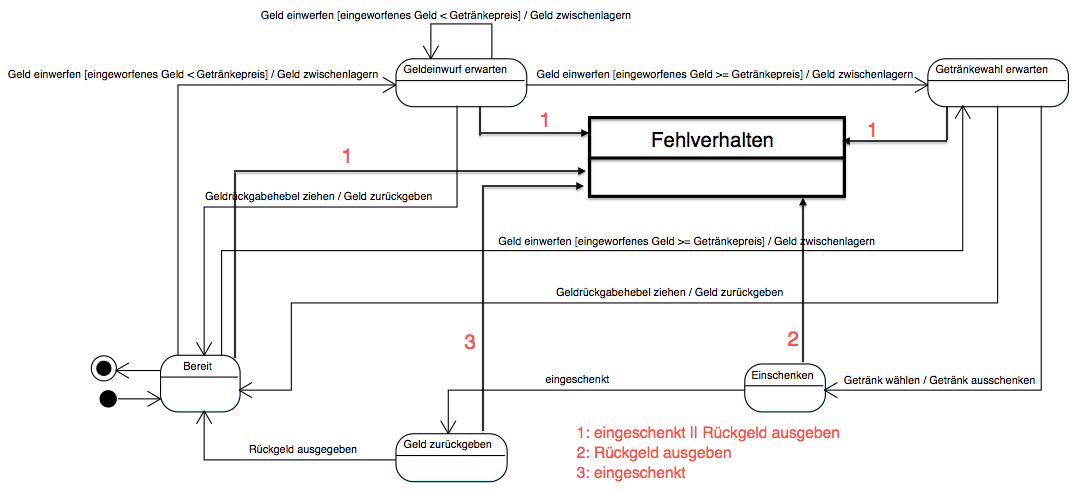
\includegraphics[width=450px]{pictures/aufg3_1.png}

  \section*{Aufgabe 3.2}
  \subsection*{(a)}
  

  \subsection*{(b)}

  \section*{Aufgabe 3.3}
  Wird zur Repr�sentation der Fliesenarten eine JAVA-Aufz�hlung (\texttt{enum}) genutzt,
  so k�nnen Testf�lle mit Fliesen aus einem anderen Material als dort definiert sind
  direkt weggelassen werden, da der Test schon im Vorfeld nicht kompilieren w�rde.\\
  Ein solcher Mechanismus wird in der Qualit�tssicherung auch als implizite
  Qualit�tssicherungsma�nahme bezeichnet.


  


\end{document}
